\documentclass[12pt]{scrreprt}
\usepackage{graphicx}
\usepackage{geometry}
\geometry{
 a4paper,
 left=20mm,
 right=20mm,
 top=25mm,
 headheight=20mm,
 headsep=0mm,
 bottom=30mm,
}
\usepackage[T1]{fontenc}				% Trennung von Umlauten.
\usepackage[ngerman]{babel}	
\usepackage[utf8]{inputenc}
\usepackage[headsepline]{scrlayer-scrpage}
\ModifyLayer[addvoffset=-10pt]{scrheadings.head.below.line}
\usepackage{blindtext}
\usepackage[font=small,labelformat=empty,justification=centering]{caption}
\setlength{\parindent}{0em}

\usepackage{svg}
\usepackage{epstopdf}

\usepackage[version=4]{mhchem}

%Autordaten
\newcommand{\datum}{16.07.2020}
\newcommand{\autorinfo}{\textbf{Wechler, Tim-Jonas} (1137877)}


\ihead{\textbf{WT 1} \datum}
\chead{\autorinfo}
\ohead{\vspace{10pt}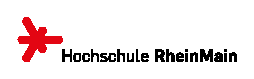
\includegraphics[width=4cm]{Logo-Hochschule-RheinMain}}
 
\begin{document}
In der letzten Vorlesung von Werkstofftechnik 1 wurden die Themen der Legierung und Normierung von Stählen behandelt.\par\medskip 

Wenn es um das Thema \textbf{Legierung} sich handelt unterscheidet man Grundlegend zwischen hochlegiertem und niederlegiertem Stahl.
\textbf{Hochlegierter} Stahl hat Sondereigenschaften wohin gegen der \textbf{niederlegierte} Stahl sich aus verschiedene Elemente zusammensetzt. Hierbei ist zu beachten das es sich mindestens um 3 Legierungselemente handelt.\par\smallskip

Ein \textbf{Legierungselement} kann die Phasenzustände stark beeinflussen und reduziert im Allgemeinen die Umwandlungsgeschwindigkeit. 
Es ist zu beachten das sich Legierungselemente gegen seitig nicht in ihren Eigenschaften aufsummieren. Viel mehr gibt es eine überproportionale Auswirkung der Eigenschaften. Es kann auch passieren das sich die Elemente in ihren Eigenschaften gegenseitig beeinflussen und schwächen. 
Um von einem Legierungselementen sprächen zu können muss ein gewisser Grenzwert überschritten sein. Ist dieser nicht überschritten, so redet man von einem Begleiter. 
Der Grenzwert ist abhängig vom Werkstoff um den es geht. Im Allgemeinen liegt der Grenzwert bei einem prozentualen Anteil von $0,05\%$. Es gibt hier noch einige Stoffe die einen Abweichenden Wert haben. 
Dieser Grenzwert kann von $1,6\%$ bei Mangang bis $0,0008\%$ bei Bor gehen. Des weiteren sind  Kohlenstoff, Phosphor, Schwefel, Stickstoff und Sauerstoff keine Legierungselemente.\par\smallskip

Bei der \textbf{Normierung} wurden uns das Thema in Form von mehreren Beispielen näher gebracht. Seit 1992 gibt es eine DIN-Norm (DIN EN 10 020) nach dem Stahl gekennzeichnet wird. 
In der Zeit vor 1992 hatte jedes Land seine eigene Normierung. Da in jedem Land die es andere Schwerpunkte gab, nach denen man normiert hatte, konnte man die Normierungen nicht immer vergleichen. 
Desweiteren dachte man führer noch anders über Werkstoff als es heute der Fall ist. Im Skript zur Vorlesung Werkstofftechnik 1 von Dr. E. Geberth kann man sich die unterschiede zwischen alt und neu anschauen. Zu dem findet man hier eine genaue Erklärung was die einzelne Teile des Normierung bedeuten. \par\smallskip

In meiner Arbeitszeit bei Müller Mitteltal GmbH habe ich mit verschiedene Stählen gearbeitet. Am häufigsten habe ich mit den Stählen S420MC, S355MC, S235JR und ein Stahl der Firma SSAB mit dem Namen Hardox 450. 
Leider konnte ich hierzu keine Normierung finden. Dem Datenblatt kann man nur die chemische Zusammensetzung, den Kerbschlagwert und weitere Toleranzen entnehmen. Das Datenblatt läst sich auf der Seite \\
https://www.ssab.de/produkte/warenzeichen/hardox/hardox-product-overview finden. \par\medskip

Um abschließend über das gelernte ein letztes Wort zu verlieren, fand ich es interessant über die Grenzwerte und das Verhalten von Legierungselementen zu erfahren. Auch fand ich es sehr interessant mein bisheriges Wissen der unterschiedlichen Stählen mit dem Wissen der Vorlesung zu verknüpfen. Leider habe ich keine Normierung für den letzten Stahl finden können. Dennoch war es Aufschlussreich das Datenplatt zu lesen. 


\end{document}
